\section{Results}
One of the test scenarios used during development of the algorithm is the navigation through a 1km by 1km square section of the city of Leuven, Belgium. This data is freely available from the local government \footnote{\url{https://overheid.vlaanderen.be/producten-diensten/basiskaart-vlaanderen-grb}} and represents a real life scenario. Not all of the buildings in the dataset have a convex shape. The algorithm only handles convex obstacles, so the convex hull of each building is used. This area contains 3079 distinct buildings, ranging between 4 and well over 10 vertices per building. The path that needs to be planned is about 1.3km long. Figure \ref{fig:example} shows a visualization of the path and many other elements that go into calculating it.
\\
The grid size for Theta* is set at 5m, yielding a 200 by 200 grid. Calculating the initial path takes around 30 seconds. From this path, 21 segments are constructed. Each segments takes on average just under 11 seconds to solve, although the time to solve each segment ranges from 0.3s to 74s. The final path consists of 960 distinct timesteps at 10Hz, although significantly more have been calculated to ensure the vehicle can reach its goal in each segment within the given amount of timesteps for that segment.
\begin{figure*}[!t]
    \centering


    \subfloat{
        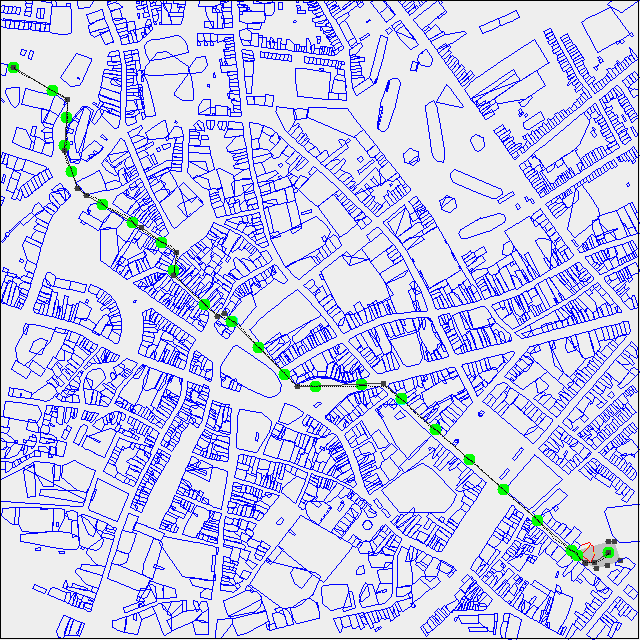
\includegraphics[width=0.2\textwidth]{img/leuven}
    }
    \hfil
     \subfloat{
        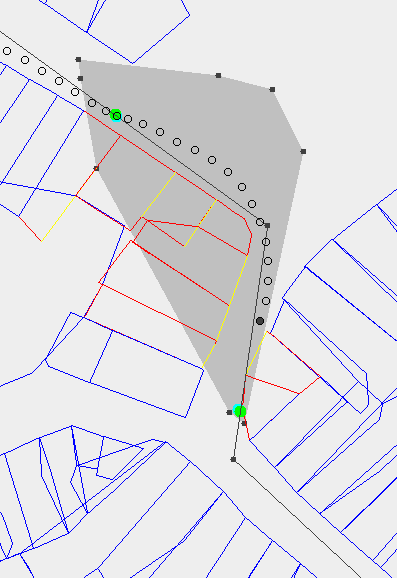
\includegraphics[width=0.2\textwidth]{img/zoomed}
     }

    \caption{The left image shows an overview of the 1km by 1km map, and the path from the top-left to the bottom-right. The right image shows a zoomed-in view of a part of the path. The blue polygons are buildings. The black segmented line is the initial Theta* path. The filled green circles represent the transitions between segments. The dark gray region on the right shows the active region, with the active obstacles in red and yellow. The current position of the vehicle is represented by the filled gray circle, while its position in the timesteps leading up to the current timestep are represented by the hollow gray circles.}\label{fig:example}
\end{figure*}
\\
MILP path planning has not been demonstrated on a scale like this before. This technique can also scale even further. Given an initial path, the complexity of the algorithm scales roughly linearly with the amount of segments. The main bottleneck that prevents this approach from scaling up further is the Theta* step. By replacing Theta* with a more efficient implementation, or an entirely different algorithm, larger scales can be achieved.

\section{Conclusion}